\documentclass[dvisvgm,multi=true]{standalone}
\usepackage{mathmlcoresvg}
\begin{document}
% <figcaption><span>Figure 16: </span>Box model for the <code>roundedbox</code>
  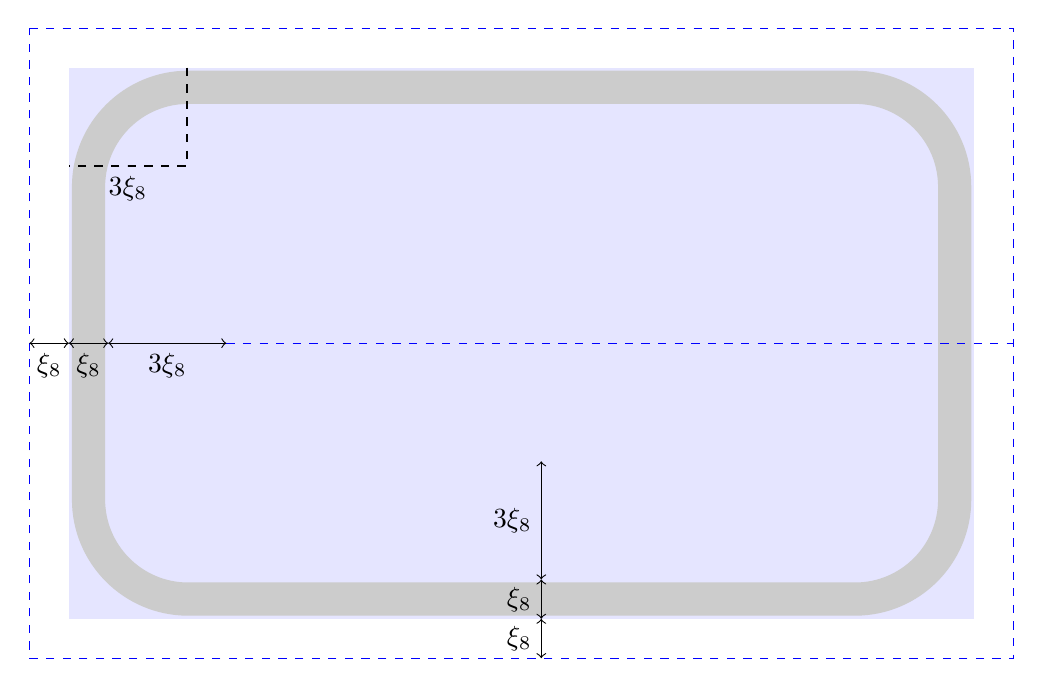
\begin{tikzpicture}[yscale=-1]

  \fill[blue!10]
  (-2,-3.5) -- (9.5,-3.5) -- (9.5,3.5) -- (-2,3.5) -- cycle;

  \MathMLBox{0}{0}{1.5}{1}{red};

  \draw[black!20,line width=12,rounded corners=36]
  (-1.75,-3.25) -- (9.25,-3.25) -- (9.25,3.25) -- (-1.75,3.25) -- cycle;

  \draw[dashed,blue]
  (-2.5,-4) -- (10,-4) -- (10,4) -- (-2.5,4) -- cycle
  (0,0) -- (10,0);

  \draw[<->] (0,0) -- (-.75,0)node[below]{$3\xi_8$} -- (-1.5,0);
  \draw[<->] (-1.5,0) -- (-1.75,0)node[below]{$\xi_8$} -- (-2,0);
  \draw[<->] (-2,0) -- (-2.25,0)node[below]{$\xi_8$} -- (-2.5,0);

  \draw[<->] (4,1.5) -- (4,2.25)node[left]{$3\xi_8$} -- (4,3);
  \draw[<->] (4,3.5) -- (4,3.25)node[left]{$\xi_8$} -- (4,3);
  \draw[<->] (4,3.5) -- (4,3.75)node[left]{$\xi_8$} -- (4,4);

  \draw[dashed](-.5,-3.5) --
  (-.5,-2.25) -- (-1.25,-2.25)node[below]{$3\xi_8$} -- (-2,-2.25);

\end{tikzpicture}

\end{document}
